\section{System Architecture}\label{arch}
Now, we overview the \sys architecture, its goals, and describe how our framework integrates with existing data cleaning solutions.

\subsection{Overview}
The primary goal of \sys is to provide a framework that wraps around existing Machine Learning and Data Cleaning systems.
Instead of cleaning the entire data upfront and then training a model, we initialize the framework with a model, and iteratively correct it with small batches of clean data.
Built into the framework are feedback mechanisms that use information from the cleaning to improve performance on future batches of clean data.

There are two basic operating modes of \sys: (1) error detection oracle and (2) adaptive error detection. 
These two modes differ in the way they partition dirty and clean data, where (1) assumes we can differentiate the two in advance, and (2) assumes we can learn it from samples.
Partitioning serves two purposes: (1) it reduces the variance of our updates because we can cheaply scan over data we know that is clean, and (2) it increases the fraction of actually dirty records in the candidate batch.
A good example of why we need the second objective is seen in the context of crowdsourcing.
If we have a crowdworker clean records, we will have to pay them for the task whether or not the record required cleaning.
Partitioning has important ramifications since classifiying erroneous data as cleaned can impart a bias on our model.
We will overview how the architecture and applications change based on these modes.

First, we overview our notation and terminology:

\vspace{0.5em}

\noindent \textbf{Featurization: } Given a relation $R$ with a set of attributes $A$.
There is a featurization function $F$ which maps every row in $\mathcal{R}$ to a $d$ dimensional feature vector and a $l$ dimensional label tuple: 
\[F(r \in \mathcal{R}) \mapsto (\mathbb{R}^l, \mathbb{R}^d)\]
The result of the featurization are the data matrices $X$ and $Y$.
\[
F(R)\rightarrow (X,Y)
\]
We consider problems in which the training examples (i.e., rows in the data matrix) have a one-to-one relationship with rows in the base data ($R$).

\vspace{0.5em}

\noindent\textbf{Initialization: } To initialize \sys, the user gives us the base dirty relation $R$, the featurization $F$, and a dirty model $\theta^{(d)}$ that is derived from the dirty relation. So initially $\theta^{(1)} = \theta^{(d)}$

\vspace{0.5em}

\noindent\textbf{Error Detection: } The first step in \sys is error detection. In this step, we select a candidate set of dirty records $R_{dirty} \subseteq R$.  

\vspace{0.5em}

\noindent\textbf{Error Sampling: } The second step in \sys is sampling. Since we cannot clean all of the dirty records, we take a sample of the records $S_{dirty} \subseteq R_{dirty}$.

\vspace{0.5em}

\noindent\textbf{Error Repair: } Next, we apply a repair procedure $C$ to the sample of data $S_{dirty}$ to get a clean sample $S_{clean}$. Given a dirty record $r$, the error repair module applies a repair $C$ to the record, to return $C(r)\mapsto r_{clean}$. 

\vspace{0.5em}

\noindent\textbf{Model Update: } Then, we update the model $\theta^({(i)})$ based on the newly cleaned data $F(S_{clean})$. The result is the updated model $\theta^({(i+1)})$.

\vspace{0.5em}

\noindent\textbf{Error Impact Estimate: } Based on the change between $F(S_{clean})$ and $F(S_{dirty})$, we direct the next iteration of sampling to select points that will have changes most valuable to the next model update.

\subsubsection{Error Detection Oracle}
For many types of errors, it is possible to efficiently enumerate a set of corrupted records and enumerate what is wrong with these records.
For example, in example \ref{exm-1}, this is the set of records with missing values and we know exactly which attributes (and corresponding features) are corrupted.
We describe these types of errors as having an \emph{error detection oracle}.
In Figure \ref{sys-arch4a}, we add more detail to our introductory architecture diagram when we are applying \sys to such errors.

\begin{figure}[t]
\centering
 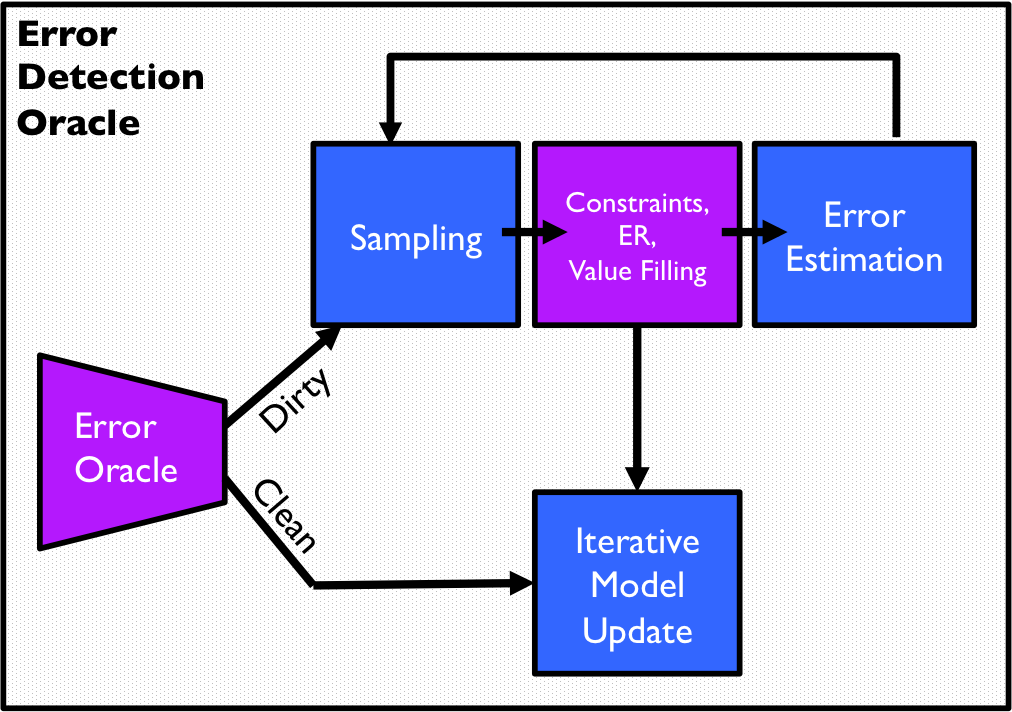
\includegraphics[width=0.6\columnwidth]{figs/arch1a.png}
 \caption{We detail the \sys architecture when we are using an error detection oracle. In this model, we have a way to enumerate all the records that are dirty before running any cleaning. \label{sys-arch4a}}
\end{figure}

\begin{enumerate}
\item Initialize with a dirty model $\theta^{(1)} = \theta^{(d)}$, batch size $b$, and number of iterations $T$
\item Error Detection. In the first step, we use the oracle to select a set of records $R_{dirty}$.
Associated with each $r \in R_{dirty}$ is a set of errors $e_r$ which tells us which features are corrupted.
For example, if a missing value in attribute $a$ affects features $\{1,2,6\}$, then $e_r=\{1,2,6\}$.
The error detection step gives us the following tuple: $(R_{dirty},E_r)$.

\item For each iteration $i=1,...,T$

\begin{enumerate}
\item Error Sampling. We sample a batch of records from $R_{dirty}$ each record has a sampling probability $p_i$. (Described in Section \ref{model-update})
\item Error Repair. We apply the user-specified data cleaning $C(S_{dirty})$
\item Model Update. We use the results of the cleaning to update the model $\theta^{(i+1)}$ (Described in Section \ref{model-update}).
\item Error Impact Estimate. Based on the results of the cleaning, we update $p_i$ to guide the data cleaning to the most valuable data (Described in Section \ref{sampling}).
\end{enumerate}
\item Return $\theta^{(T+1)}$
\end{enumerate}

\noindent We highlight example use cases of this architecture using data cleaning methodologies proposed in the liteature.

\vspace{0.5em}

\noindent\textbf{Constraint-based Repair: }
One model for handling errors in database declaring a set of constraints on a database and 
iteratively fixing records such that the constraints are satisfied \cite{DBLP:journals/pvldb/YakoutENOI11, DBLP:journals/pvldb/FanLMTY10, khayyat2015bigdansing}.
However, automatically repairing can be unreliable \cite{DBLP:journals/pvldb/FanLMTY10}.
Recently proposed systems like Guided Data Repair \cite{DBLP:journals/pvldb/YakoutENOI11}, use human input to validate suggested fixes.

\vspace{0.5em}

\emph{Error Detection. } Let $\Sigma$ be a set of constraints on the relation $\mathcal{R}$. 
In the error detection step, we select a subset of records $\mathcal{R}_{dirty} \subseteq \mathcal{R}$ that violate at least one constraint.
The set $e_r$ is the set of columns for each record which have a constraint violation.

\vspace{0.5em}

\emph{Error Repair. } \sys supports both automated and human validated data repair for constraints. For automated techniques, we can apply the record-level ``local" repair proposed in \cite{DBLP:journals/pvldb/FanLMTY10} or we can use human corrections as in \cite{DBLP:journals/pvldb/YakoutENOI11}. 

\begin{example}
Consider our EEG data running example, for an example of constraint-based cleaning.
We can add a constraint that one of the electrical signals cannot be greater than 4V.
For all records whose value is above 4V, we would select them in the error detection step.
Then, in the error repair step, we could apply a repair that sets the erroneous signal value to its most likely value.
\end{example}

\vspace{0.5em}

\noindent\textbf{Entity Resolution: }
Another common data cleaning task is Entity Resolution \cite{gokhale2014corleone, DBLP:journals/pvldb/KopckeTR10, wang2012crowder}.
A common pattern in Entity Resolution is to split up the operation into two steps: blocking and matching.
In blocking, attributes that should be the same are coarsely grouped together.
In matching, those coarse groups are resolved to a set of distinct entities.
Increasingly the matching step is done by crowd workers \cite{wang2012crowder, gokhale2014corleone}, leading to very expensive costs.

\vspace{0.5em}

\emph{Error Detection. } This is the matching step. Let $S$ be a similarity function that takes two records and returns a value in $[0,1]$ (1 most similar and 0 least similar). For some threshold $t$, $S$ defines a similarity relationship between two records $r$ and $r'$:
\[
r \approx r' : S(r,r') \ge t
\] 
In the error detection step, $R_{dirty}$ is the set of records that have at least one other record in the relation that satisfy $r \approx r'$.
The set $e_r$ is the attributes of $r$ that have entity resolution problems.

\vspace{0.5em}

\emph{Error Repair. } \sys supports both automated and human validated entity resolution for resolving a set of matches to a single entity.

\begin{example}
An example of an Entity Resolution problem is where the patient's gender is inconsistently represented (e.g., ``Male", ``M", ``Man"). 
We can define a similarity relationship $(\text{first char =} 'M')$ and select all records that satisfy this condition.
In the error repair step, a human can fix the inconsistencies setting all records that meet the condition to the canonical value.
\end{example}

\subsubsection{Adaptive Detection}
The second operating mode of \sys is adaptive detection.
In this mode, the analyst does not know the set of errors in advance but learns them as she cleans more data.
Consider the case when she has to do exploratory data analysis to discover the errors.
In Figure \ref{sys-arch4b}, we add more detail to our introductory architecture diagram when we are applying \sys to such errors.

\begin{figure}[t]
\centering
 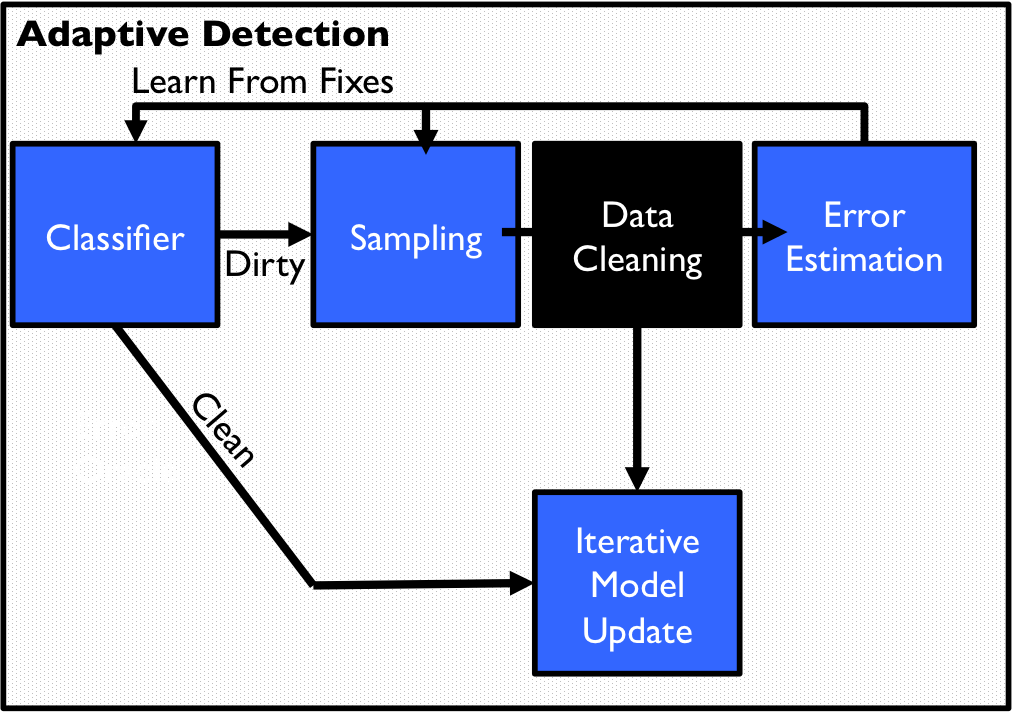
\includegraphics[width=0.6\columnwidth]{figs/arch1b.png}
 \caption{We detail the \sys architecture when we are using adaptive detection. In this model, we do not assume that we can enumerate the set of erroneous records in advance. \label{sys-arch4a}}
\end{figure}

\begin{enumerate}
\item Initialize with a dirty model $\theta^{(1)} = \theta^{(d)}$, batch size $b$, number of iterations $T$, and $R_{dirty} = R$
\item For each iteration $i=1,...,T$
\begin{enumerate}
\item Error Sampling. We sample a batch of records from $R_{dirty}$ each record has a sampling probability $p_i$. (Described in Section \ref{model-update})
\item Error Repair. We apply the user-specified data cleaning $C(S_{dirty})$
\item Model Update. We use the results of the cleaning to update the model $\theta^{(i+1)}$ (Described in Section \ref{model-update}).
\item Error Impact Estimate. Based on the results of the cleaning, we update $p_i$ to guide the data cleaning to the most valuable data (Described in Section \ref{sampling}).
\item We maintain a classifier to prune the set of dirty records based on what was cleaned.
\end{enumerate}
\item Return $\theta^{(T+1)}$
\end{enumerate}

\noindent We highlight an example use case of this architecture.

\vspace{0.5em}

\noindent\textbf{Interactive Data Cleaning with OpenRefine.}
\begin{example}
Consider our analyst using an interative tool such as OpenRefine \cite{openrefine} to clean her data. 
She takes a sample of data from the entire dataset.
She then uses the tool to determine which records are corrupted and dirty.
As she marks more records as dirty, the system learns what features determines a dirty record.
This classifier can be used to guide cleaning in future batches of data.
\end{example}

\subsection{Designing for Expensive Repair}
This framework is designed around data cleaning operations where the expensive step is error repair.
It is well known that most constraint-based error repair problems are NP-Hard.
As the complexity of errors increases, so does the amount of computation needed to resolve them.
The consequence is that automated repair is either not scalable or relies on greedy repairs that can be unreliable.
Increasingly, human effort is seen as unavoidable in data cleaning \cite{park2014crowdfill, wang2012crowder, gokhale2014corleone, wang1999sample} either due to the cost of formulating constraints, scripting fixes for all possible errors, or in actually cleaning the data.

When humans are involved, per record latencies for data repair are orders of magnitude larger than the CPU time needed for numerical operations.
In CrowdFill \cite{park2014crowdfill}, processing 20 rows of data required 10 minutes 54 secs.
Likewise, in CrowdER \cite{wang2012crowder}, the median crowd task finished in 58secs.
These latencies severly limit the scale of these systems. 
Even in highly optimized distributed automated systems such as BigDansing, data cleaning required 7700 seconds for 3M rows.
Data cleaning is fundementally slow in comparison to the CPU time needed for numerical vector operations.
In contrast, a model training framework like CoCoA (implemented on Spark like Big Dansing), requires on the order of minutes to train a 3M row model \cite{jaggi2014communication}.

Based on current data cleaning trends, we argue that model training will be orders of magnitude faster than data repair.
We aggressively optimize our system for this design point, where we clean a very small fraction of data.
This leads to new problems and opportunities in non-uniform sampling, partitioning, and integrated model training-cleaning.

\iffalse
\subsection{Optimizations}
There are three aspects of \sys, that allow us to achieve this design point: error partitioning, gradient-based model update (Section \ref{model-update}), estimate-driven sampling (Section \ref{sampling}).

\vspace{0.5em}

\noindent\textbf{Partitioning Dirty and Clean Data: } In many applications, enumerating the set of corrupted records is much easier than cleaning them. For example, we may be able to select the set of rows that have missing values but actually filling those missing values is expensive. Likewise, in the constraint literature, selecting a set of rows that have a violated constraint can be done in polynomial time, however, fixing the constraints is NP-Hard.
In our error detection step, we partition the dirty and clean data.
Partitioning serves two purposes: (1) it reduces the variance of our updates because we can cheaply scan over data we know that is clean, and (2) it increases the fraction of actually dirty records in the candidate batch.
A good example of why we need the second objective is seen in the context of crowdsourcing.
If we have a crowdworker clean records, we will have to pay them for the task whether or not the record required cleaning.
To efficiently use this partitioning, we need a database solution indexing dirty and clean data.

\vspace{0.5em}

\noindent\textbf{Gradient-Based Updates: } In \sys, we start with a dirty model and then make an update using a gradient step. Here, we can draw an analogy to Materialized View maintenance, since after all, a model parametrized by $\theta$ is just a table of floating point numbers.
Krishnan et al. proposed a technique called sample view cleaning, in which they take a clean sample of data and propagate the updates to a Materialized View.
Similarly, in this work, we take the information from a sample of cleaned data and propagate an update with the gradient.

\vspace{0.5em}

\noindent\textbf{Estimate-Driven Sampling: } Repair is the most expensive step in the workflow, so optimizing for scan cost may lead to negligible overall time improvements.
We can sacrifice a small overhead in pre-computation for each data point to determine its value to the model and select a sampling distribution accordingly.
Intuitively, while each iteration has an increased cost, it also makes more progress towards the optimum.
\fi


